\documentclass[aspectratio=169]{beamer}

\usepackage[T1]{fontenc}
\usepackage[utf8]{inputenc}
\usepackage{lmodern}
\usepackage{amsmath,amssymb}
\usepackage{booktabs}
\usepackage{tikz}
\usetikzlibrary{positioning, arrows.meta}

\usetheme{Madrid}
\usecolortheme{seahorse}
\setbeamertemplate{navigation symbols}{}
\setbeamertemplate{footline}[frame number]

\title{Clustered Federated Learning (CFL)}
\subtitle{Aprendizado federado clusterizado, divisivo, com o cosseno entre atualizações}
\author{luiz2801}
\institute{Repositório \texttt{cfl\_stocfl}}
\date{Baseado em Sattler, Müller e Samek (2021)}

\begin{document}

\begin{frame}
  \titlepage
\end{frame}

\begin{frame}{Roteiro}
  \begin{enumerate}
    \item Problema: dados não-IID e um único modelo global
    \item Ideia do CFL: clusters de clientes, um modelo por cluster
    \item Quando dividir: os critérios de norma
    \item Como dividir: bipartição pelo cosseno
    \item O algoritmo prático e o cenário do notebook
    \item Correções feitas no repositório e limitações
  \end{enumerate}
\end{frame}

\section{Problema}

\begin{frame}{Federated Learning e heterogeneidade}
  \begin{itemize}
    \item Clientes treinam localmente e enviam só atualizações de pesos.
    \item O servidor agrega com FedAvg: média dos pesos dos clientes.
    \item Se os clientes têm distribuições diferentes (não-IID), um único
      modelo global serve mal a todos.
  \end{itemize}

  \vspace{0.6em}
  \begin{block}{Exemplo}
    Um cliente vê dígitos rotacionados 180\textdegree{} e outro não. A média
    dos dois modelos não resolve bem nenhum dos dois casos.
  \end{block}
\end{frame}

\begin{frame}{Suposições do artigo}
  \begin{itemize}
    \item Há $M$ clientes, e o cliente $i$ tem dados $D_i$ de uma distribuição $\varphi_{I(i)}$.
    \item A função $I$ (cliente $\rightarrow$ distribuição) e o número $K$ de distribuições são
      \textbf{desconhecidos} do servidor.
    \item \textbf{Suposição 1 (FL):} existe um $\theta^*$ que minimiza, ao mesmo tempo, o risco
      de todos os clientes. Quando isso vale, os clientes são \emph{congruentes}.
    \item \textbf{Suposição 2 (CFL):} existe uma partição dos clientes em grupos que satisfazem a
      Suposição 1.
  \end{itemize}
\end{frame}

\section{Ideia do CFL}

\begin{frame}{Ideia central}
  \begin{itemize}
    \item O CFL não altera o protocolo de FL. Continua havendo rodadas de FedAvg.
    \item A diferença é que o servidor observa as atualizações $\Delta W_i$ e decide
      \emph{quando} e \emph{como} separar os clientes em clusters.
    \item Cada cluster continua seu próprio FedAvg, e clusters só se dividem.
  \end{itemize}
\end{frame}

\begin{frame}{Abordagem divisiva (top-down)}
  \begin{center}
    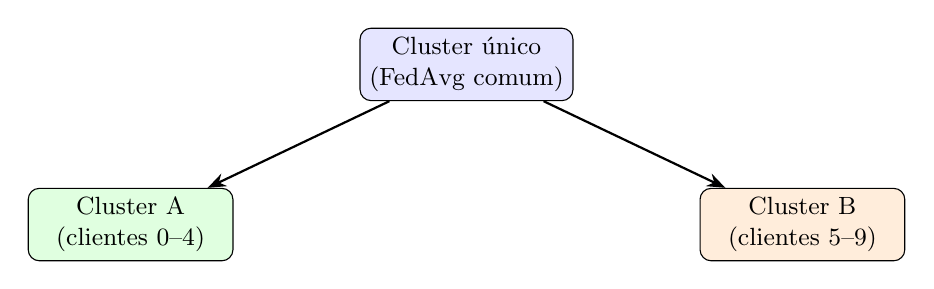
\begin{tikzpicture}[
      node/.style={draw, rounded corners, align=center, font=\small, minimum width=2.6cm, minimum height=0.9cm},
      edge/.style={-{Stealth}, thick}]
      \node[node, fill=blue!10] (r) {Cluster único\\(FedAvg comum)};
      \node[node, fill=green!12, below left=1.1cm and 1.6cm of r] (a) {Cluster A\\(clientes 0--4)};
      \node[node, fill=orange!14, below right=1.1cm and 1.6cm of r] (b) {Cluster B\\(clientes 5--9)};
      \draw[edge] (r) -- (a);
      \draw[edge] (r) -- (b);
    \end{tikzpicture}
  \end{center}
  \vspace{0.3em}
  \begin{itemize}
    \item Começa com um único cluster com todos os clientes.
    \item Uma divisão acontece somente quando os critérios indicam clientes incongruentes.
  \end{itemize}
\end{frame}

\section{Quando dividir}

\begin{frame}{Dois critérios de norma}
  Seja $\Delta W_i$ a atualização do cliente $i$ no cluster $c$.
  \begin{align*}
    \text{média:}\quad & \mathrm{mean\_norm} = \left\| \sum_{i \in c} \frac{|D_i|}{|D_c|}\, \Delta W_i \right\|
      \quad \text{(perto de um estacionário do FL)}\\[0.6em]
    \text{máximo:}\quad & \mathrm{max\_norm} = \max_{i \in c} \| \Delta W_i \|
      \quad \text{(algum cliente ainda está longe do seu ótimo)}
  \end{align*}
  \vspace{0.4em}
  \begin{block}{Condição para considerar a divisão}
    $\mathrm{mean\_norm} < \varepsilon_1 \quad \text{e} \quad \mathrm{max\_norm} > \varepsilon_2$
  \end{block}
\end{frame}

\begin{frame}{Intuição}
  \begin{itemize}
    \item Clientes congruentes: o gradiente de cada um também vai a zero, e a norma máxima cai.
    \item Clientes incongruentes: o FedAvg chega a um ponto em que os gradientes se
      \emph{cancelam} na média. Mas cada cliente continua longe do seu próprio ótimo.
    \item Resultado: $\mathrm{mean\_norm}$ pequeno com $\mathrm{max\_norm}$ grande indica
      incongruência.
  \end{itemize}
\end{frame}

\section{Como dividir}

\begin{frame}{Bipartição pelo cosseno}
  \begin{itemize}
    \item Calcula-se a matriz de similaridade de cosseno entre os $\Delta W_i$ do cluster.
    \item O Algoritmo 1 do artigo ordena os pares do mais parecido ao menos parecido e
      funde grupos até restarem dois. É equivalente a \emph{single linkage}.
    \item Seja $\alpha^{\max}_{\text{cruz}}$ o maior cosseno entre clientes de lados opostos.
  \end{itemize}
  \vspace{0.6em}
  \begin{block}{Critério de aceitação}
    A divisão só é aceita se
    \[
      \gamma_{\max} < \sqrt{\frac{1 - \alpha^{\max}_{\text{cruz}}}{2}}
    \]
    em que $\gamma_{\max}$ é um limite assumido, não estimado dos dados.
  \end{block}
\end{frame}

\begin{frame}{Por que o cosseno separa os clientes}
  \begin{itemize}
    \item Com duas distribuições, num ponto estacionário:
      \[
        0 = a_1 \nabla R_1(\theta^*) + a_2 \nabla R_2(\theta^*)
      \]
    \item Se os gradientes não são nulos, eles têm \textbf{direções opostas} entre os grupos.
      O cosseno vale $+1$ dentro de um grupo e $-1$ entre grupos, no caso sem ruído.
    \item Com dados finitos há ruído, e o Teorema da Separação dá a condição de $\gamma_{\max}$.
  \end{itemize}
  \vspace{0.4em}
  \small Teorema e condição de aceitação: seção 3.9.2 do guia técnico.
\end{frame}

\section{Algoritmo prático}

\begin{frame}{Algoritmo 5 do artigo (o implementado)}
  Cada rodada, para cada cluster $c$ no servidor:
  \begin{enumerate}
    \item Calcula $\Delta\theta_c = \frac{1}{|c|}\sum_{i \in c} \Delta\theta_i$.
    \item Se $\|\Delta\theta_c\| < \varepsilon_1$ e $\max_i \|\Delta\theta_i\| > \varepsilon_2$,
      calcula os cossenos entre os $\Delta\theta_i$ e a bipartição $(c_1, c_2)$.
    \item Calcula $\alpha^{\max}_{\text{cruz}}$.
    \item Divide somente se $\gamma_{\max} < \sqrt{(1 - \alpha^{\max}_{\text{cruz}})/2}$.
  \end{enumerate}
  \vspace{0.4em}
  Os clientes usam o \textbf{mesmo} modelo do cluster e, opcionalmente, uma permutação
  ortonormal $P$ trocada entre eles, para preservar a privacidade.
\end{frame}

\begin{frame}{Valores de referência}
  \begin{itemize}
    \item Recomendação do artigo: $\varepsilon_1 \approx \tfrac{1}{10}\max_t \|\Delta\theta_c\|$.
    \item $\varepsilon_2 \in [\varepsilon_1,\, 10\,\varepsilon_1]$.
    \item No notebook: $\varepsilon_1 = 0{,}2$, $\varepsilon_2 = 0{,}8$ ($\varepsilon_2/\varepsilon_1 = 4$) e
      $\gamma_{\max} = 0{,}5$.
    \item A regra de $\varepsilon_1$ daria $0{,}03$ a $0{,}04$, abaixo do que o ruído do SGD permite,
      então o valor foi recalibrado. As normas dependem de taxa de aprendizado, épocas e arquitetura.
  \end{itemize}
\end{frame}

\section{Implementação}

\begin{frame}{Arquivos do projeto}
  \small
  \begin{tabular}{@{}ll@{}}
    \toprule
    Arquivo & Conteúdo \\
    \midrule
    \texttt{clustered\_federated\_learning.ipynb} & Experimento completo (ponto de entrada) \\
    \texttt{fl\_devices.py} & \texttt{Client}, \texttt{Server}, operações sobre pesos e similaridade \\
    \texttt{data\_utils.py} & Partição Dirichlet não-IID \\
    \texttt{models.py} & \texttt{ConvNet} para EMNIST (62 classes) \\
    \texttt{helper.py} & Logger do experimento e gráficos \\
    \bottomrule
  \end{tabular}
  \vspace{0.6em}

  \footnotesize Pasta do projeto: \texttt{projetos/clustered-federated-learning/}
\end{frame}

\begin{frame}{Cenário do notebook}
  \begin{itemize}
    \item EMNIST (byclass), com 10 mil amostras de treino e 10 mil de teste.
    \item 10 clientes, com dados não-IID por partição Dirichlet ($\alpha = 1{,}0$).
    \item Clientes 0 a 4 têm os dados rotacionados 180\textdegree{}, o que induz dois grupos.
    \item Cada cliente: 80\% treino e 20\% avaliação. SGD com taxa de aprendizado $0{,}1$.
    \item 80 rodadas, com todos os clientes participando em cada rodada.
  \end{itemize}
\end{frame}

\section{Correções e limitações}

\begin{frame}{Correções feitas no repositório}
  O código foi ajustado para seguir o texto do artigo:
  \begin{itemize}
    \item \textbf{Bug de índices na segunda divisão em diante.} A bipartição devolvia posições
      dentro do subcluster, mas eram tratadas como ids de cliente. Havia clientes duplicados ou
      ausentes. Em 12 sementes, 4 terminaram com partição inválida.
    \item Divisão pelo Algoritmo 5, com o Algoritmo 1 e a checagem de $\gamma_{\max}$.
    \item SGD puro, e os limiares foram recalibrados.
  \end{itemize}
  \vspace{0.4em}
  \small Detalhes e registro das decisões: \texttt{docs/guia.md} (seções 3.7 e 3.10) e \texttt{docs/decisoes.md}.
\end{frame}

\begin{frame}{Limitações}
  \begin{itemize}
    \item Assume que \textbf{todos} os clientes de um cluster participam em \textbf{toda} rodada.
      Não trata amostragem parcial.
    \item Divisões são irreversíveis.
    \item A passagem de gradientes para $\Delta\theta$ é heurística, sem cota explícita.
    \item O servidor aprende quão parecidos são os clientes. Não há análise formal de privacidade.
    \item A árvore de parâmetros para clientes novos (Algoritmo 4) não está implementada no notebook.
    \item O limite do teorema é de pior caso, e $\gamma_{\max}$ é assumido.
  \end{itemize}
\end{frame}

\begin{frame}{Referência}
  \begin{itemize}
    \item F. Sattler, K.-R. Müller e W. Samek. \emph{Clustered Federated Learning:
      Model-Agnostic Distributed Multitask Optimization Under Privacy Constraints.}
      IEEE Transactions on Neural Networks and Learning Systems, 32(8), 2021, pp. 3710--3722.
      arXiv:1910.01991.
  \end{itemize}
\end{frame}

\end{document}
